\documentclass[12pt,a4paper]{article}

\usepackage[utf8]{inputenc}
\usepackage[english]{babel}
\usepackage{amssymb, amsmath}
\usepackage{fullpage}
\usepackage{parskip}
\usepackage{url}
\usepackage[dvipsnames]{xcolor}
\usepackage{enumitem}
\usepackage{graphicx}

\renewcommand{\vec}[1]{\mathbf{#1}}
\newcommand{\from}{\colon}
\newcommand{\IR}{\mathbb{R}}
\newcommand{\IN}{\mathbb{N}}
\newcommand{\norm}[1]{\left\|#1\right\|}

\begin{document}
    
    %%%%%%%%%%%%%%%%%%%%%%%%%%%%%%%%%%%%%%%%%%%%%%%%%%
    Differential equations: vectorfields
    \hfill
    ELTE, autumn 2019/20
    %%%%%%%%%%%%%%%%%%%%%%%%%%%%%%%%%%%%%%%%%%%%%%%%%%
    
    
    %%%%%%%%%%%%%%%%%%%%%%%%%%%%%%%%%%%%%%%%%%%%%%%%%%
    \subsection*{Introduction}
    %%%%%%%%%%%%%%%%%%%%%%%%%%%%%%%%%%%%%%%%%%%%%%%%%%
    
    Consider the differential equation
    $\dot{x}(t) = A \, x(t)$ in $\IR^2$
    with a constant $2 \times 2$ matrix $A$.
    %
    For each point $x = (x_1, x_2)^\top \in \IR^2$,
    the vector $A \, x$ shows the direction of evolution
    starting from that point.
    
    %%%%%%%%%%%%%%%%%%%%%%%%%%%%%%%%%%%%%%%%%%%%%%%%%%
    \subsection*{Problems}
    %%%%%%%%%%%%%%%%%%%%%%%%%%%%%%%%%%%%%%%%%%%%%%%%%%
    
    Given the vectorfield $x \mapsto A \, x$,
    suggest a plausible matrix $A$.
    
    
    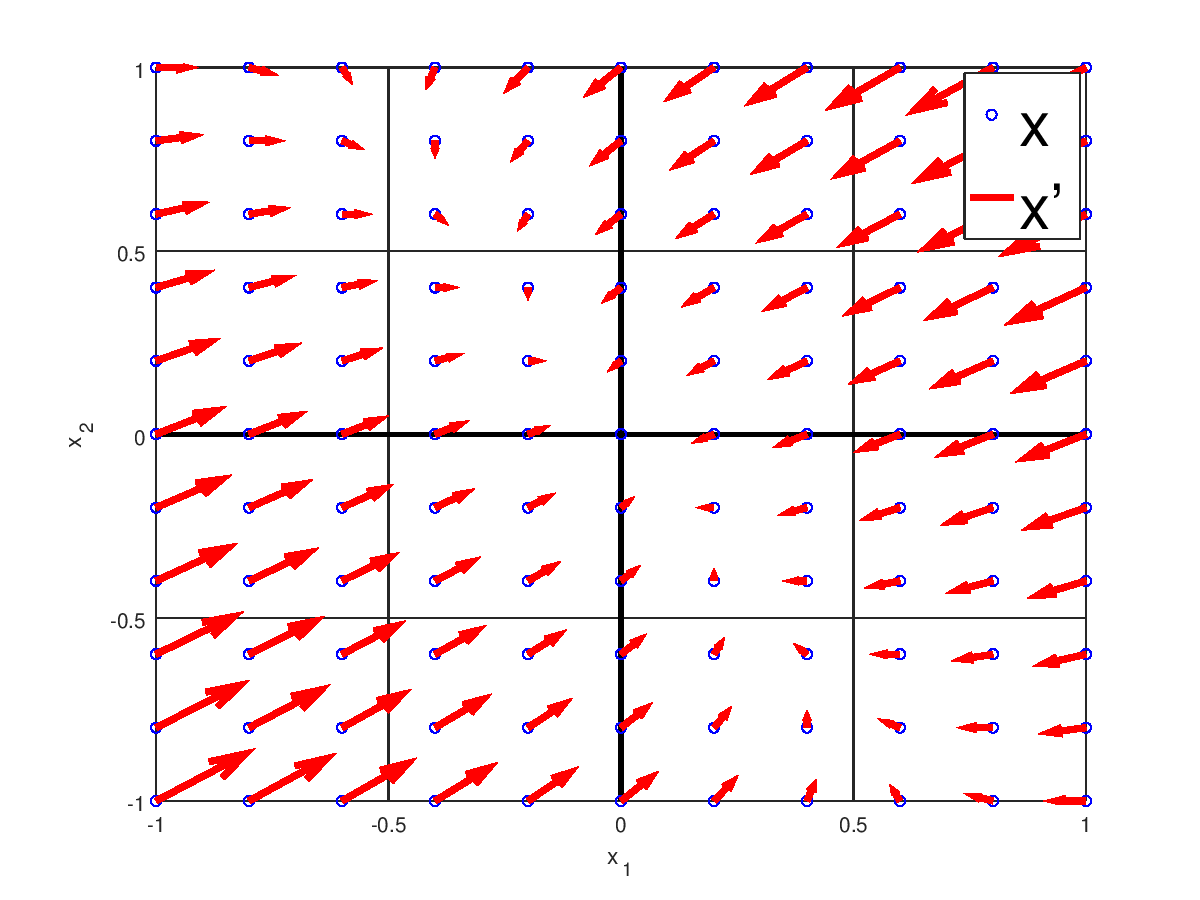
\includegraphics[width=0.25\textwidth]{A/1.png}
    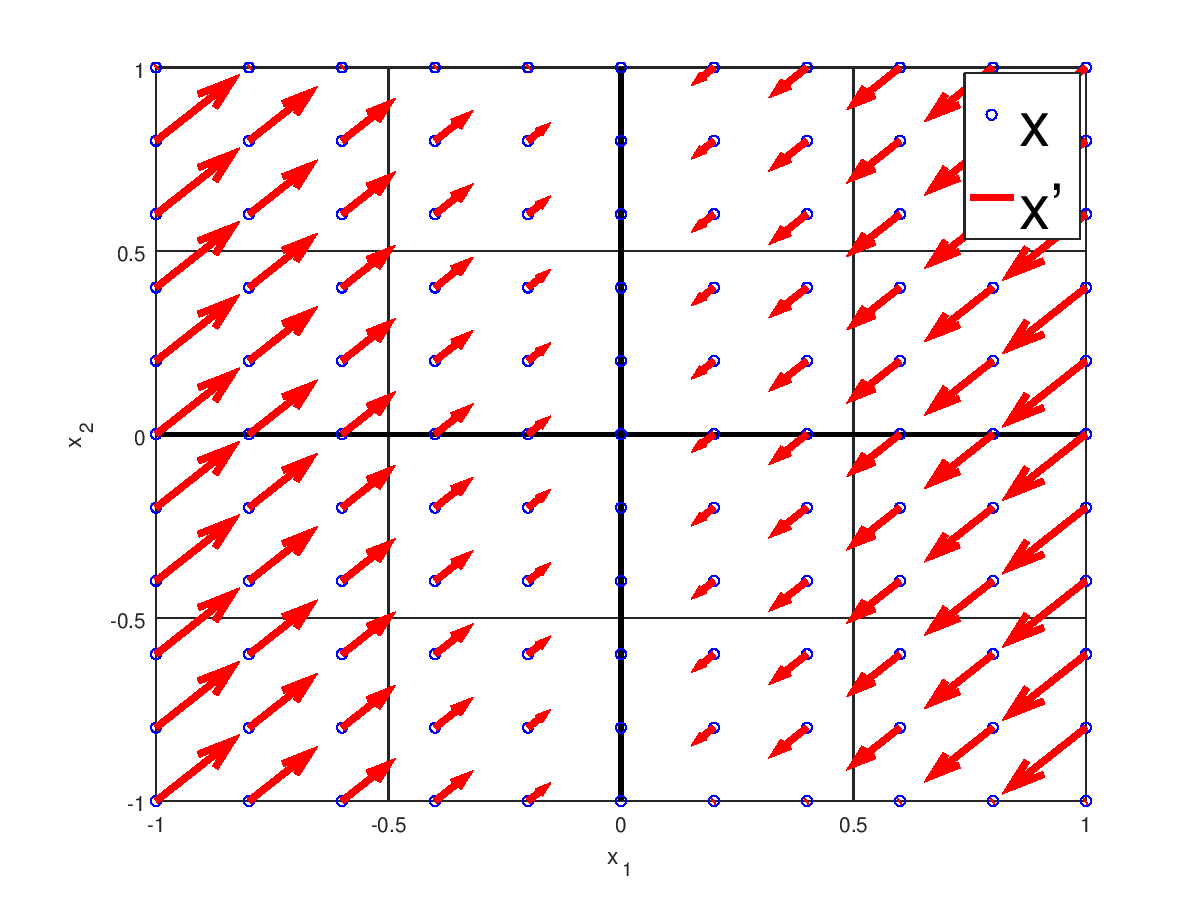
\includegraphics[width=0.25\textwidth]{A/2.png}
    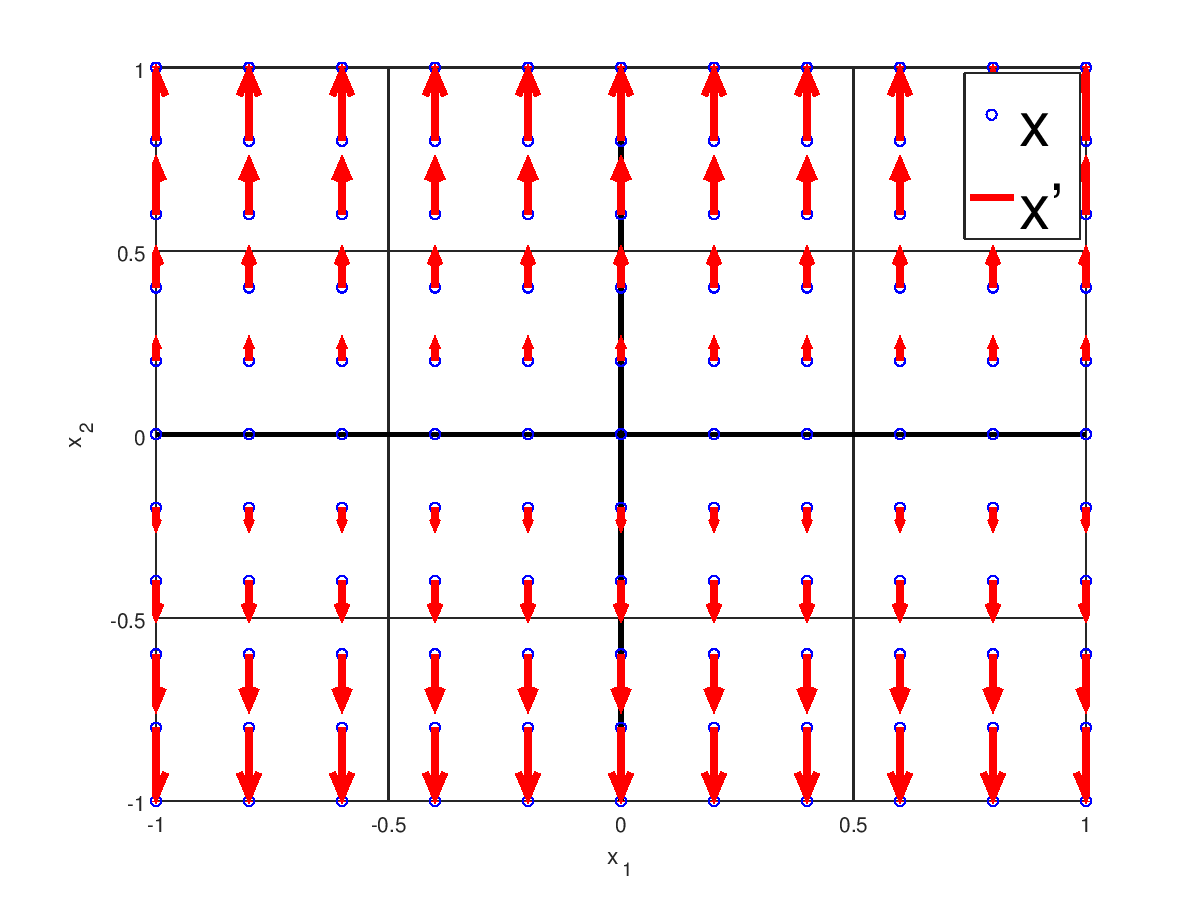
\includegraphics[width=0.25\textwidth]{A/3.png}
    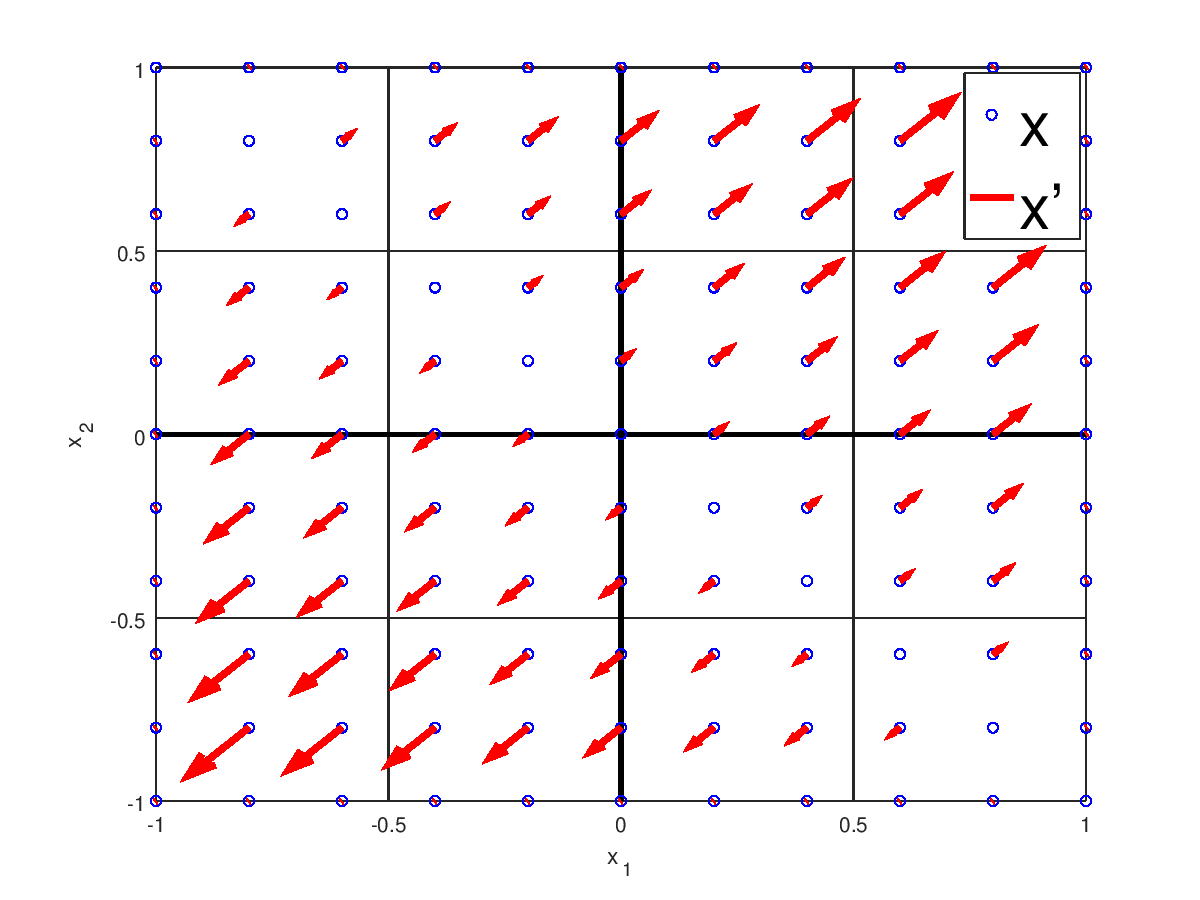
\includegraphics[width=0.25\textwidth]{A/4.png}
    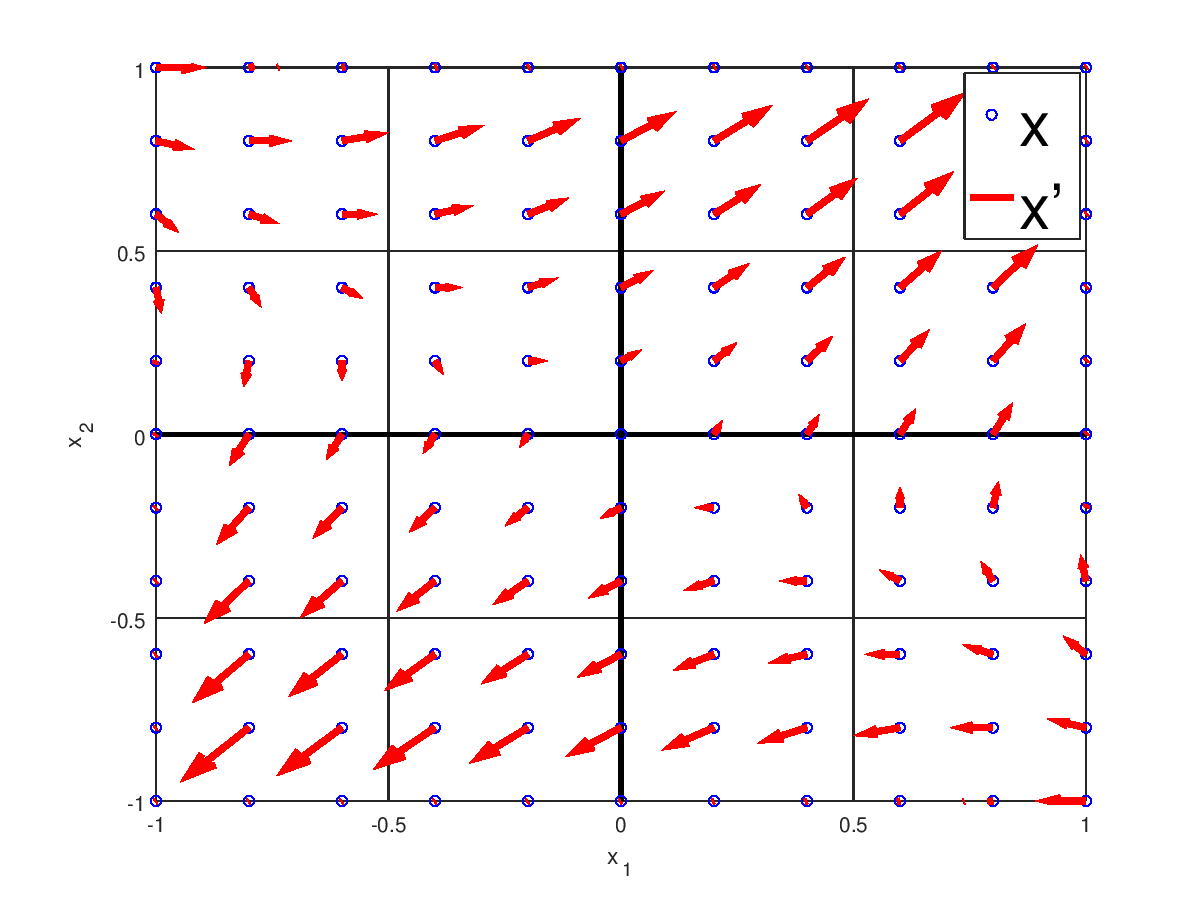
\includegraphics[width=0.25\textwidth]{A/5.png}
    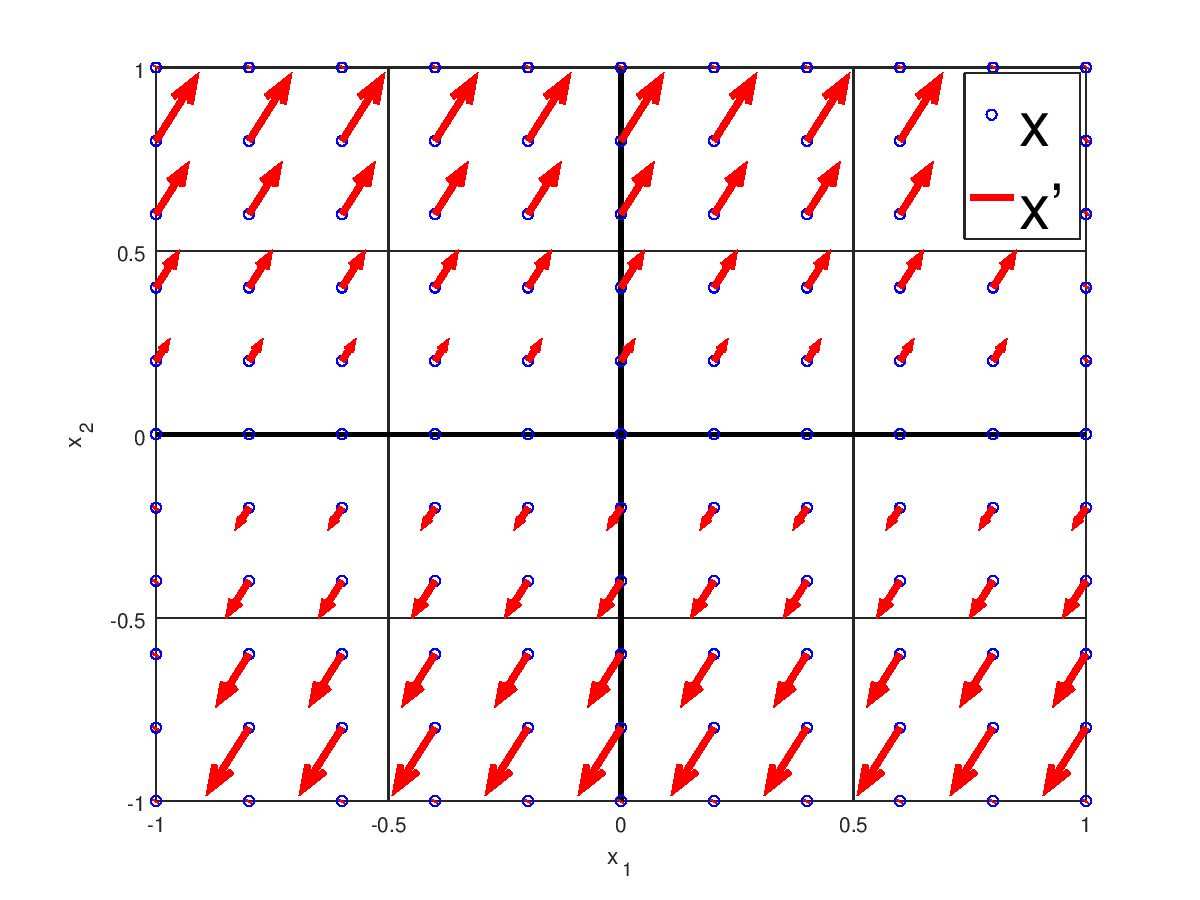
\includegraphics[width=0.25\textwidth]{A/6.png}
    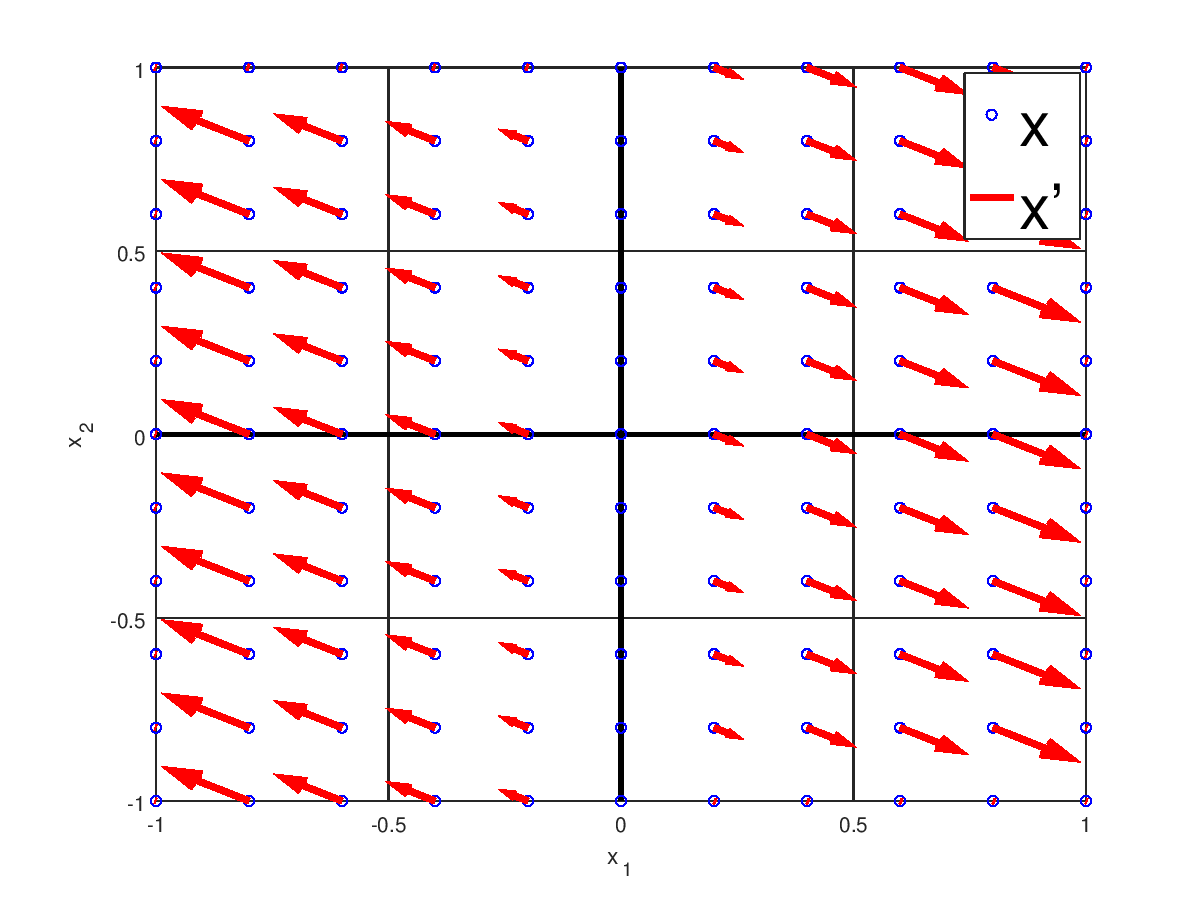
\includegraphics[width=0.25\textwidth]{A/7.png}
    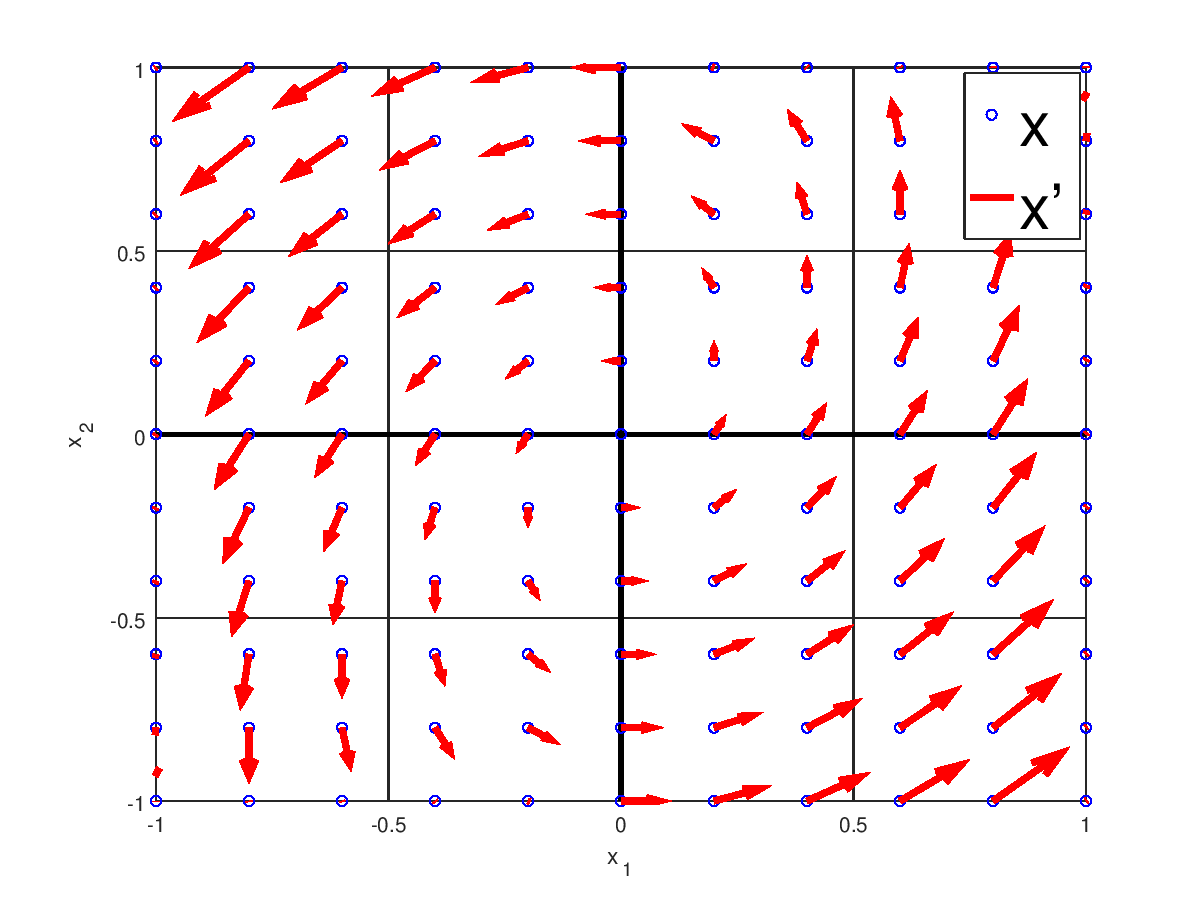
\includegraphics[width=0.25\textwidth]{A/8.png}
    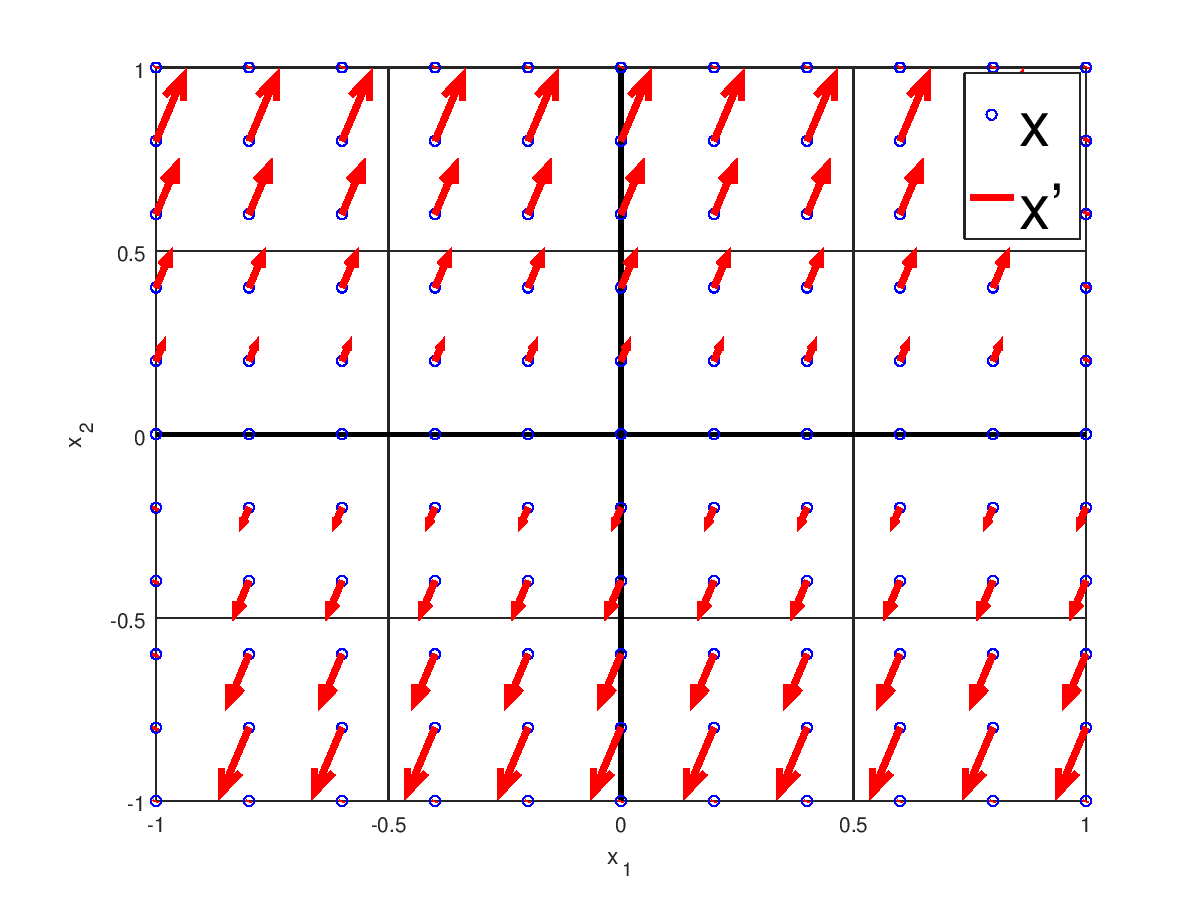
\includegraphics[width=0.25\textwidth]{A/9.png}
    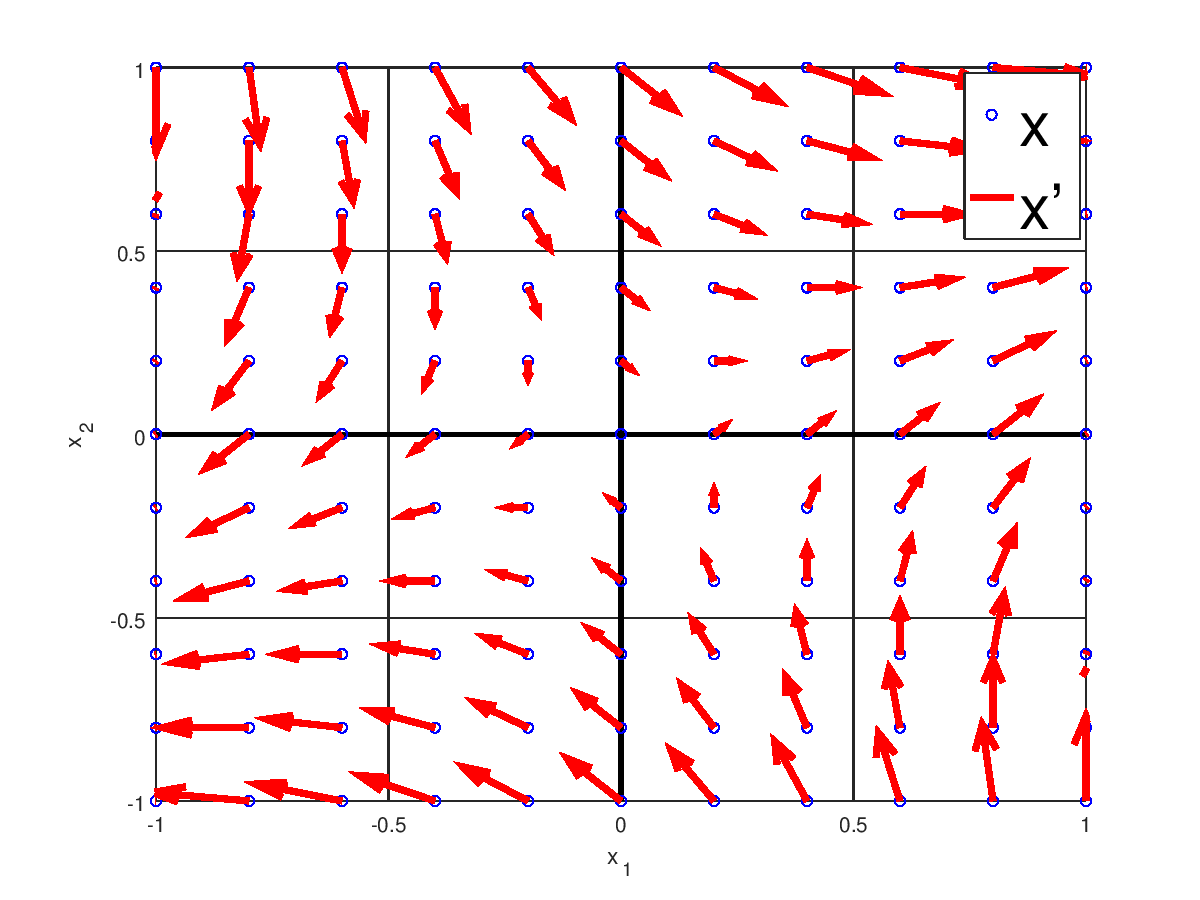
\includegraphics[width=0.25\textwidth]{A/10.png}
    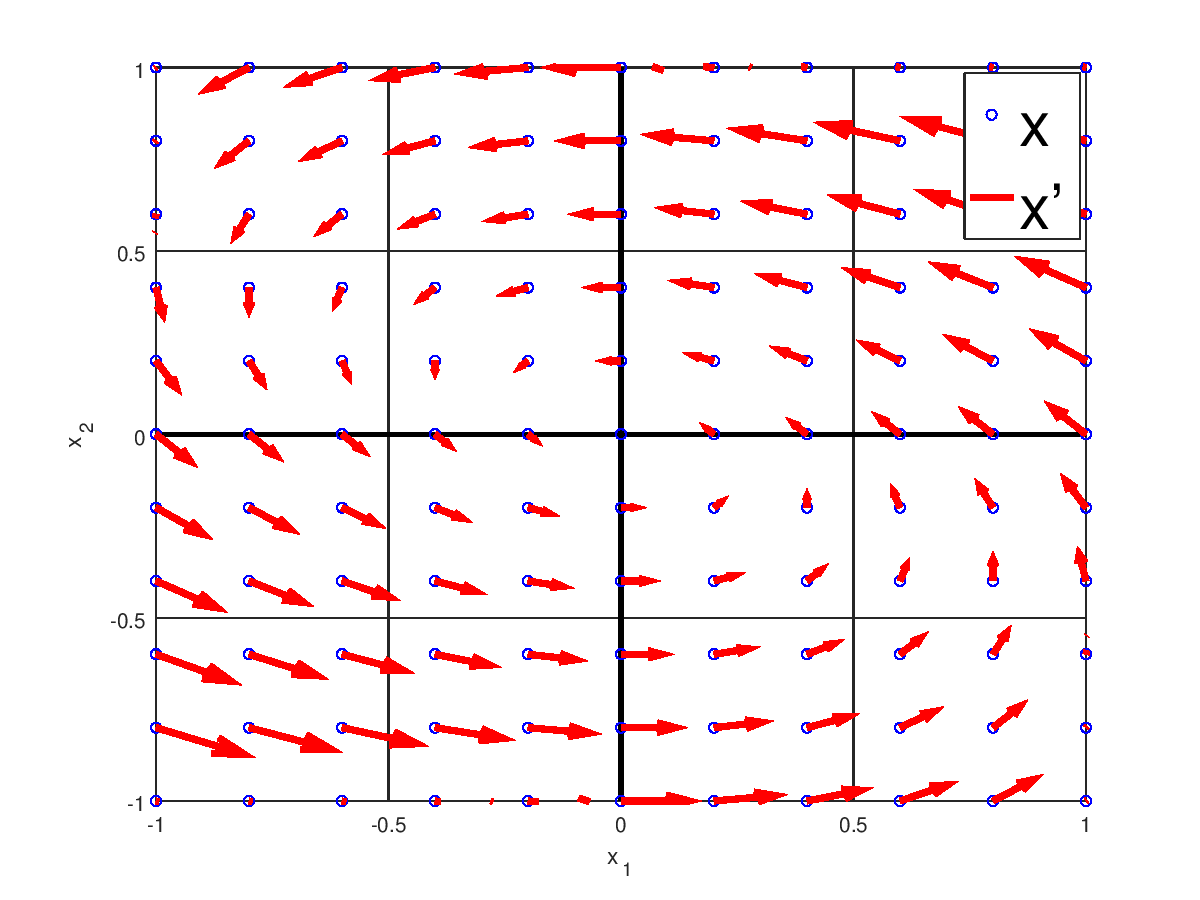
\includegraphics[width=0.25\textwidth]{A/11.png}
    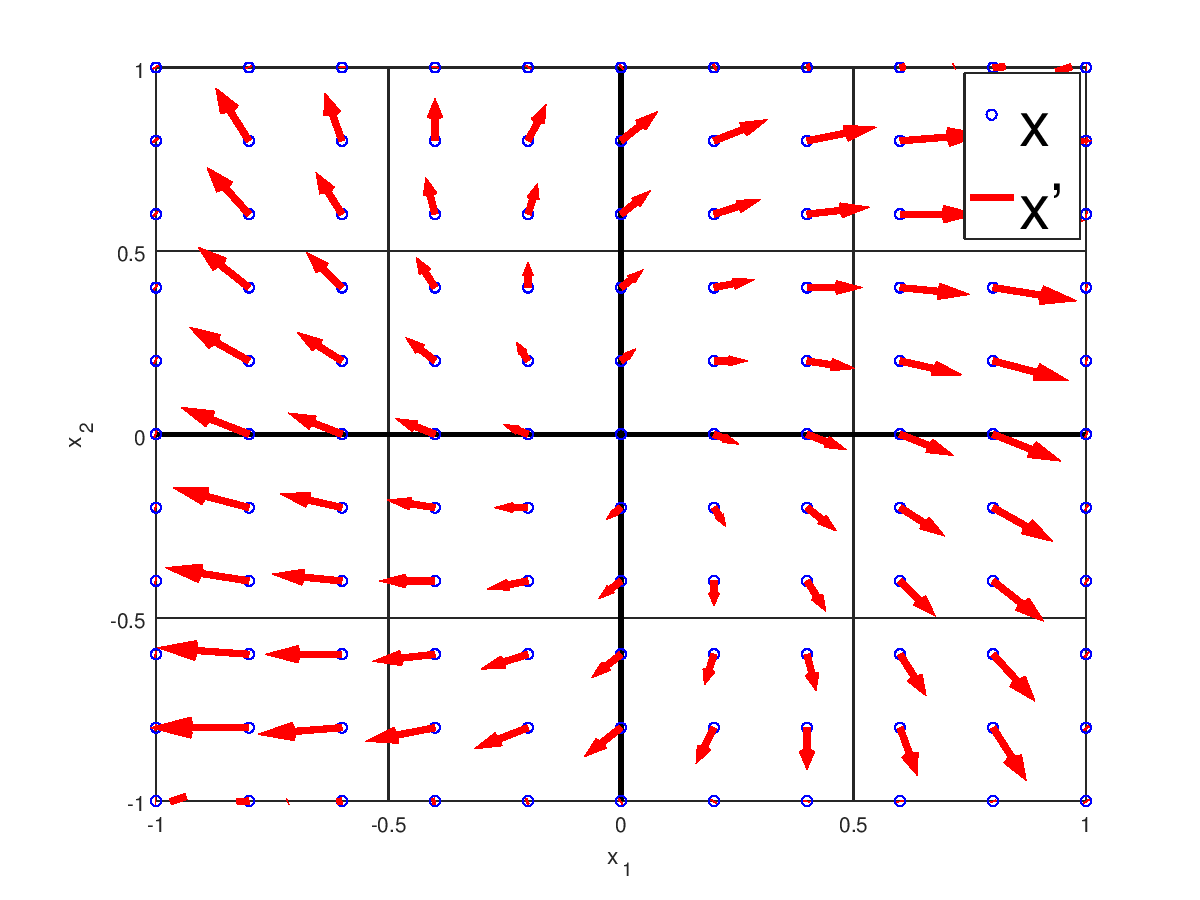
\includegraphics[width=0.25\textwidth]{A/12.png}
    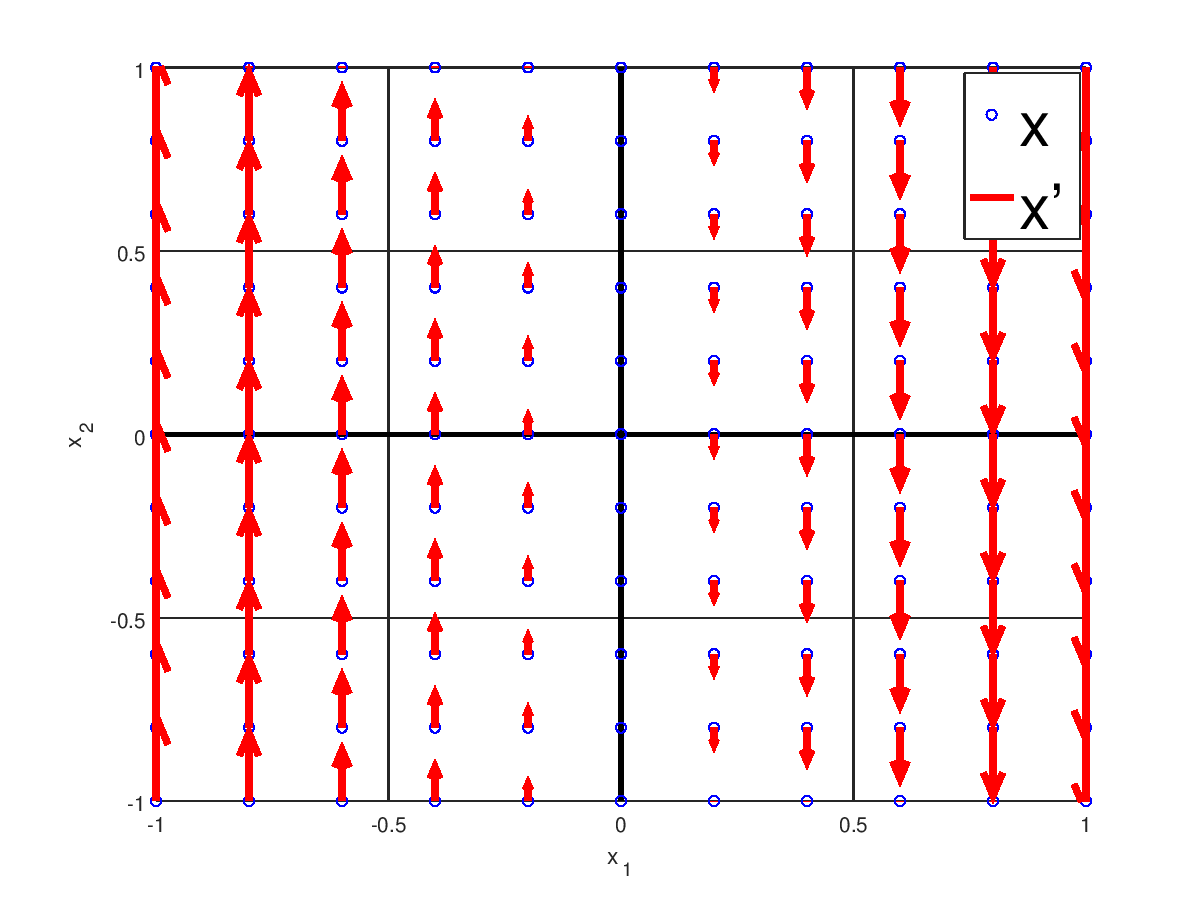
\includegraphics[width=0.25\textwidth]{A/13.png}
    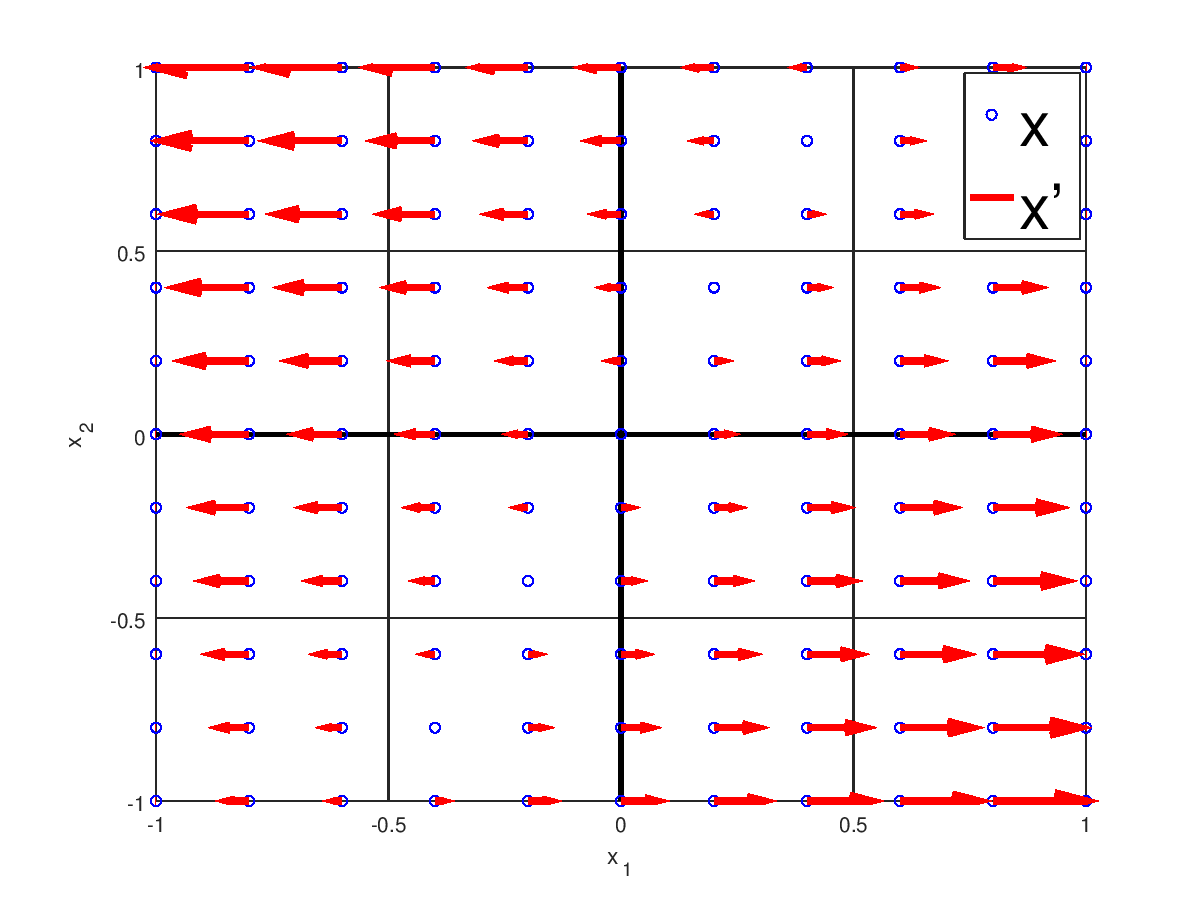
\includegraphics[width=0.25\textwidth]{A/14.png}
    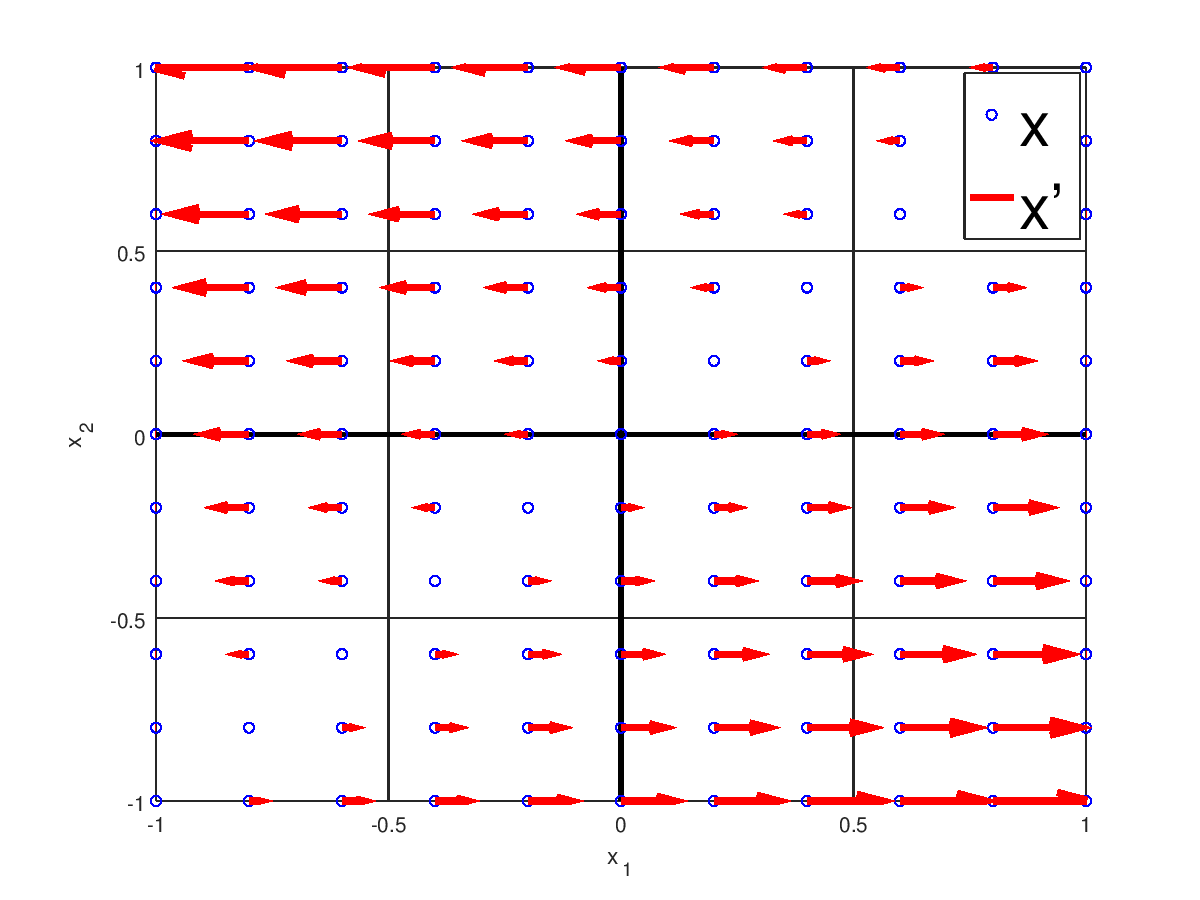
\includegraphics[width=0.25\textwidth]{A/15.png}
    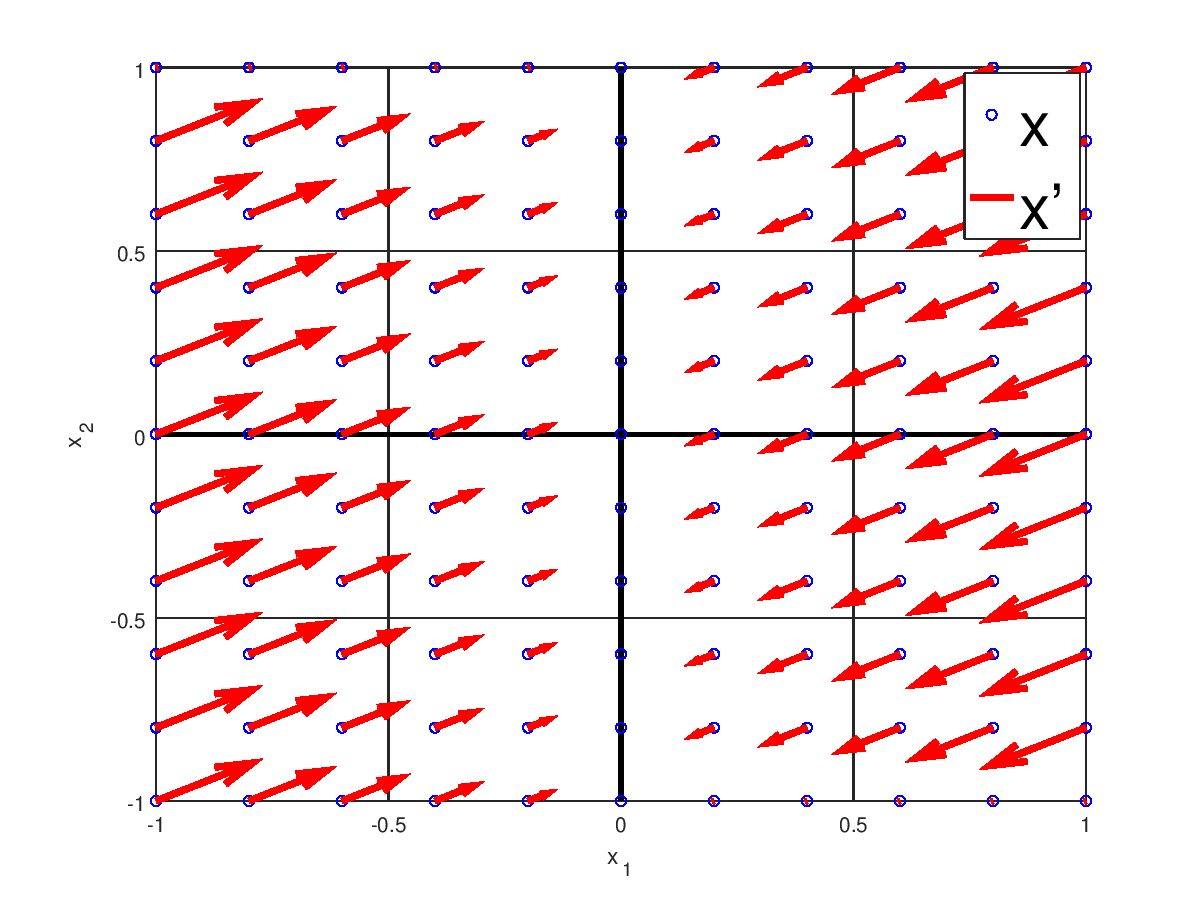
\includegraphics[width=0.25\textwidth]{A/16.png}
    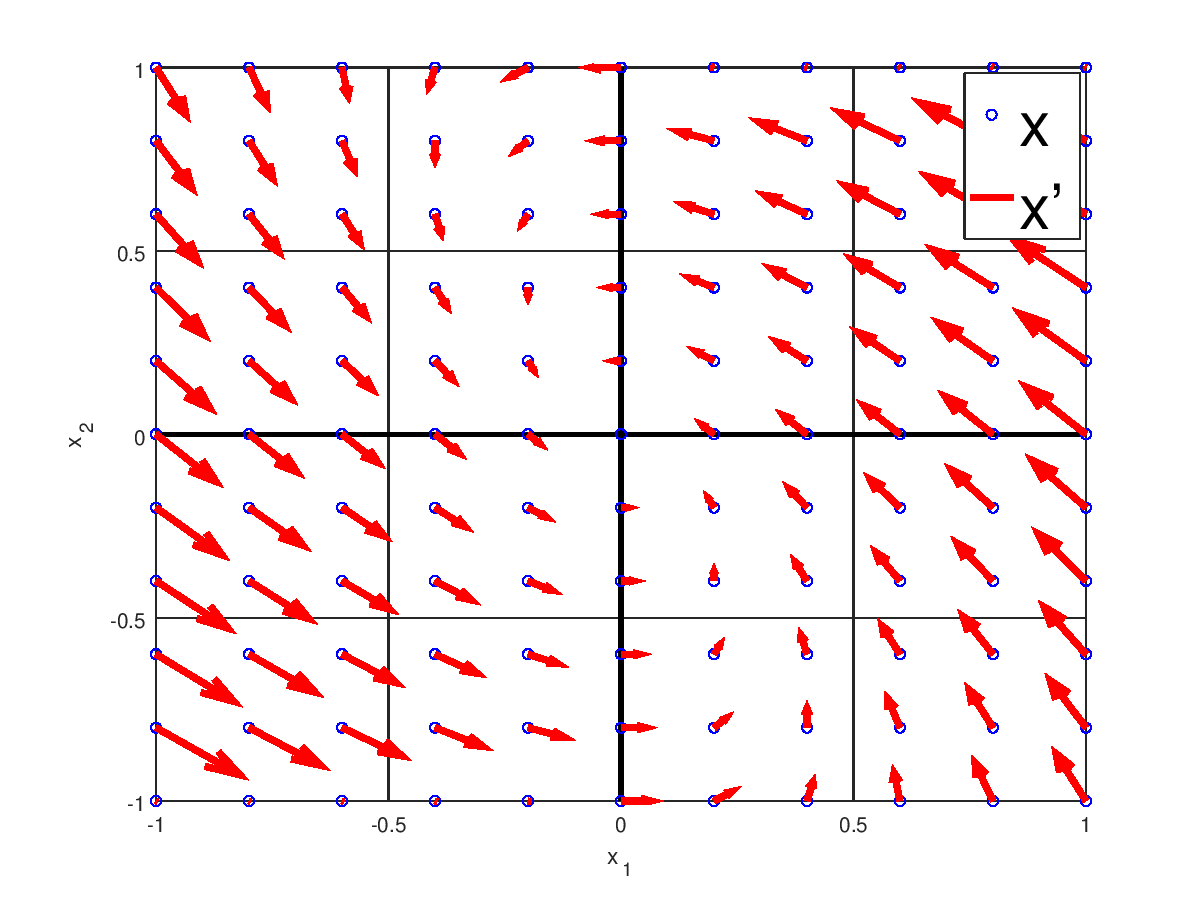
\includegraphics[width=0.25\textwidth]{A/17.png}
    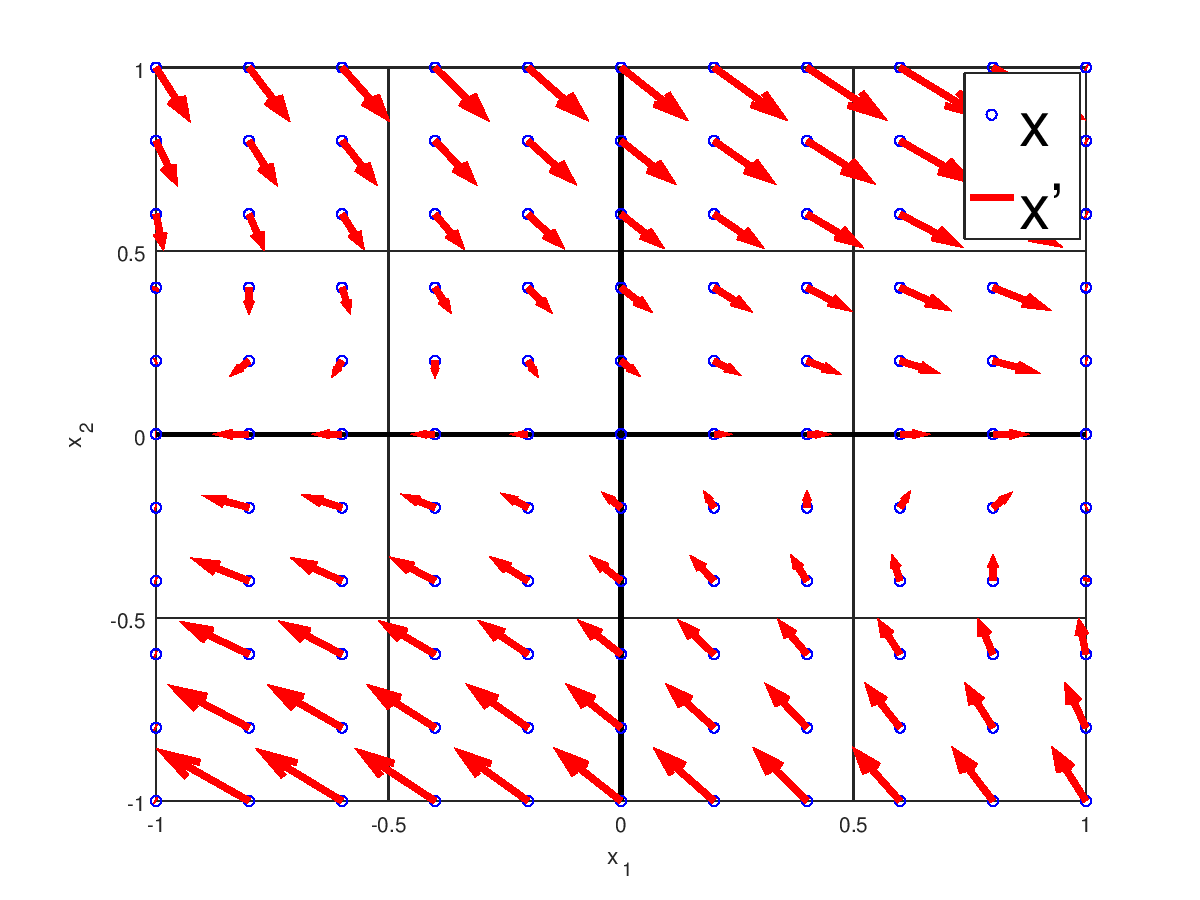
\includegraphics[width=0.25\textwidth]{A/18.png}
    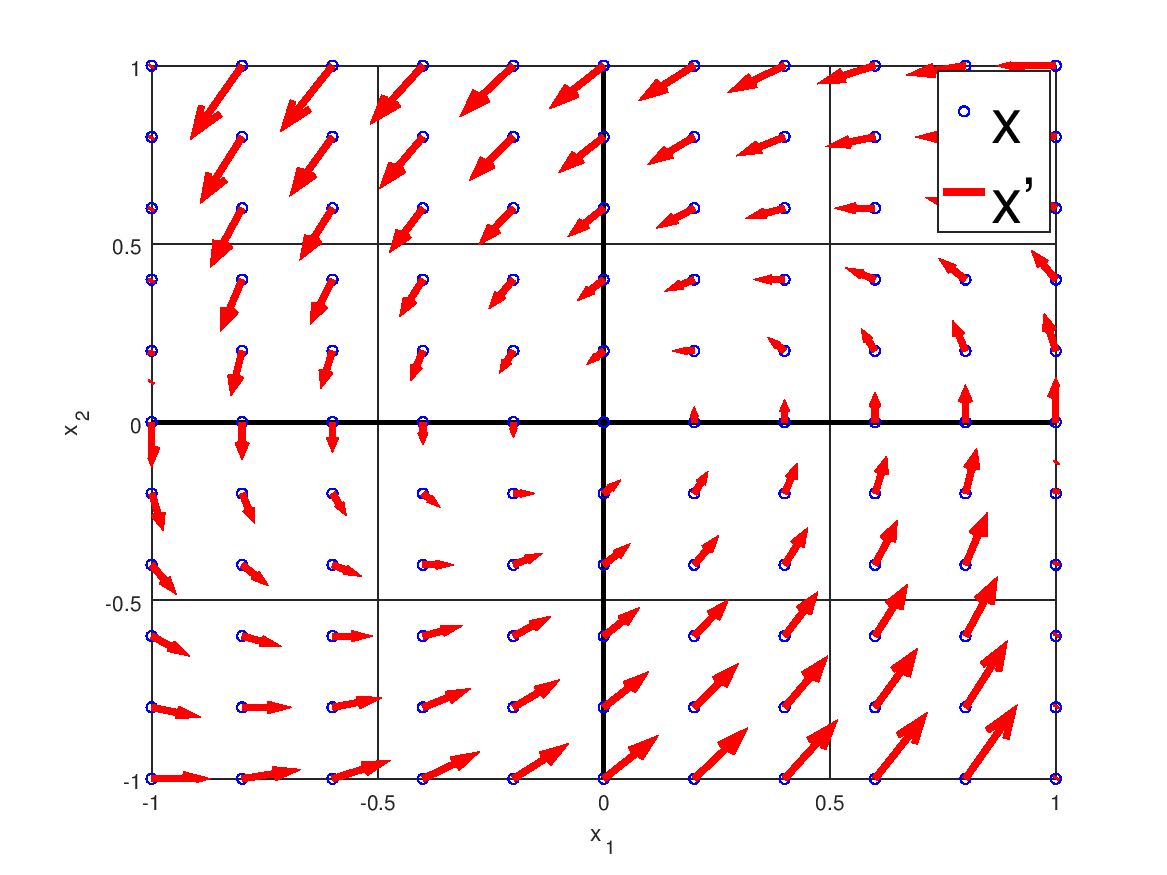
\includegraphics[width=0.25\textwidth]{A/19.png}
    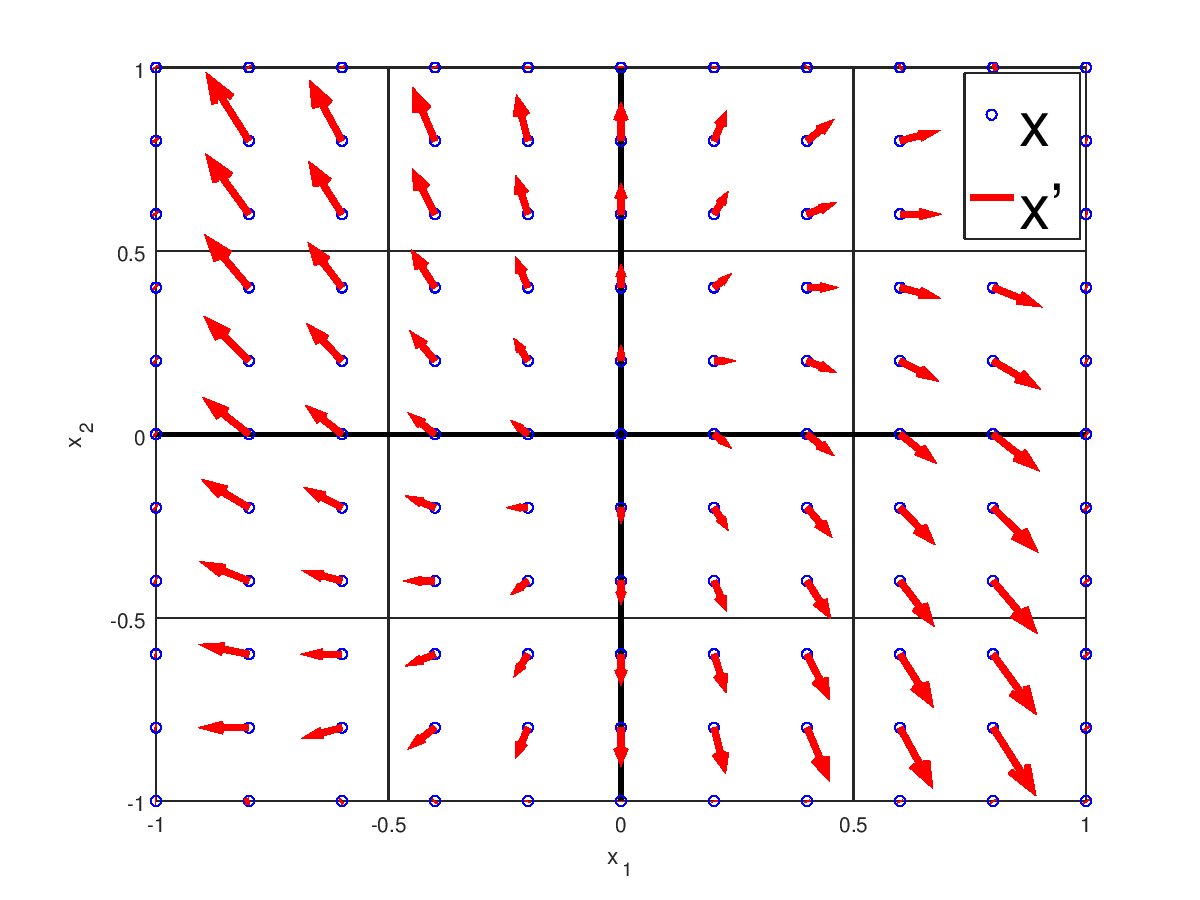
\includegraphics[width=0.25\textwidth]{A/20.png}
    
    \vfill\hfill 
    R.A., \today
\end{document}
